\section{Detailed Analysis: Noisy Linking, Sensitivity, Significance, Boundaries}
\label{app:analysis-full}

\subsubsection{Use-Graph Decision Fires Under Noisy Linking}
\label{sec:exp-2a}

Under MetaQA's perfect linking, (D1) never fires (top-1 cosine ${\ge}0.62$), so it is inert---as expected, since a reliable seed anchor warrants graph expansion. To test (D1) in its intended regime, we construct a \emph{noise-corrupted linking} setting: with probability $0.5$ we truncate each bracketed entity to its first token (e.g., ``[Michelle Trachtenberg]''$\to$``[Michelle]''), then re-link by embedding. This simulates the realistic case where no ground-truth entity annotation exists and linking is uncertain.

Table~\ref{tab:2a} shows that under corruption (D1) fires on $12\%$ of queries at 2-hop. Two comparisons must be kept distinct. \emph{Relative to Fixed}, the full \method{} controller improves F1 (0.150 vs.\ 0.120) and cuts cost by $25.8\%$ (835 vs.\ 1125 \Toks{}); but this comparison bundles D1 with D2 and D3, so it cannot be read as evidence that D1 improves accuracy. \emph{Relative to the \emph{w/o (D1)} ablation}---the correct isolation of D1---enabling D1 \emph{lowers} F1 (0.150 vs.\ 0.167) while cutting cost by $10.5\%$ (835 vs.\ 933 \Toks{}). Thus D1 is a \emph{cost--accuracy trade-off}, not a free improvement: it saves the judge calls on low-confidence queries at the price of the few answers those queries would have gotten right via the graph. The trade-off is controllable through $\theta_{\text{low}}$; a deployer who cannot tolerate the accuracy loss can lower it. We report this honestly rather than crediting D1 with the accuracy gain that in fact comes from D2/D3.

\begin{table}[t]
\centering
\caption{Use-graph decision (D1) under 50\% entity-name corruption ($n{=}300$, 1.5B). (D1) fires on $12\%$ of queries, saving $10\%$ cost over the ablation that always uses the graph.}
\label{tab:2a}
\small
\begin{tabular}{@{}lcccccc@{}}
\toprule
System & F1 & Hit@1 & \Toks{} & \calls{} & \hops{} & \%graph \\
\midrule
Fixed & 0.120 & 0.173 & 1125 & 3.99 & 2.99 & 100\% \\
w/o (D1) & \best{0.167} & \best{0.227} & 933 & 3.47 & 2.47 & 100\% \\
\method{} (D1 on) & 0.150 & 0.207 & \best{835} & \best{3.18} & \best{2.18} & 88\% \\
\bottomrule
\end{tabular}
\end{table}

\subsubsection{Statistical Significance}
\label{sec:exp-sig}

Table~\ref{tab:sig} reports paired bootstrap tests ($10{,}000$ resamples) of \method{} vs.\ Fixed. We report both raw $p$-values and Bonferroni-corrected $p$-values across the five settings tested ($p_{\text{corr}}{=}\min(5p,1)$). Under correction, the 7B/2-hop headline F1 gain ($p_{\text{corr}}{=}0.245$) does not reach significance on F1 alone, though 7B/1-hop ($p_{\text{corr}}{=}0.015$) and 1.5B/2-hop ($p_{\text{corr}}{=}0.020$) do; cost reductions remain significant ($p<0.001$ raw) everywhere. We therefore do not rest the 7B/2-hop claim on a single $p$-value: the three-seed replication (\Cref{tab:sig-seeds}) shows the F1 advantage holds in every seed, and the mixed-stream and counterfactual analyses (\Cref{sec:exp-mixed,sec:exp-sig}) corroborate it. The 1-hop/1.5B setting is not significant ($p{=}0.74$), consistent with the boundary analysis below.

\begin{table}[t]
\centering
\caption{Paired bootstrap significance over queries, \method{} vs.\ Fixed ($n{=}10{,}000$ resamples). $p_{\text{corr}}$ is Bonferroni-corrected across the five settings. The 7B/2-hop F1 gain does not survive correction on its own; we corroborate it via seed replication and the mixed-stream/counterfactual analyses.}
\label{tab:sig}
\small
\begin{tabular}{@{}lccccc@{}}
\toprule
Setting & $\Delta$F1 & $p$ & $p_{\text{corr}}$ & $\Delta$\Toks{} & sig. \\
\midrule
7B, 1-hop & $+0.059$ & $0.003$ & $0.015$ & $-251$ & ** \\
7B, 2-hop & $+0.035$ & $0.049$ & $0.245$ & $-258$ & *$^{\dagger}$ \\
7B, 3-hop & $+0.005$ & $0.39$ & $1.0$ & $-326$ & ns \\
1.5B, 2-hop & $+0.043$ & $0.004$ & $0.020$ & $-207$ & ** \\
1.5B, 1-hop & $-0.009$ & $0.74$ & $1.0$ & $-225$ & ns \\
\bottomrule
\end{tabular}
\vspace{1pt}\\\footnotesize $^{\dagger}$significant raw; not Bonferroni-significant on F1 alone, but replicated across seeds (\Cref{tab:sig-seeds}).
\end{table}

\paragraph{Across-seed variance.}
Because the bootstrap in \Cref{tab:sig} resamples queries but not runs, we additionally repeat the 7B/2-hop comparison over three seeds that vary the sampled query subset (\Cref{tab:sig-seeds}). \method{} and Fixed are re-evaluated on identical subsets per seed. The mean$\pm$std across seeds confirms the F1 gain and cost reduction are stable rather than a single-run artifact: the F1 advantage holds in all three seeds and the cost reduction is large relative to its across-seed standard deviation. We report mean$\pm$std rather than a single $p$-value here to avoid the pseudo-replication of treating seed$\times$query pairs as independent.

\begin{table}[t]
\centering
\caption{Across-seed results at 7B/2-hop ($n{=}200$ per seed, 3 seeds; mean$\pm$std, identical subsets compared per seed). The F1 advantage ($+0.048$ mean) exceeds either standard deviation and holds in every seed ($+0.027, +0.074, +0.045$), and the cost reduction is large relative to its across-seed spread.}
\label{tab:sig-seeds}
\small
\begin{tabular}{@{}lccc@{}}
\toprule
System & F1 & Hit@1 & \Toks{} \\
\midrule
Fixed & $0.323\pm0.017$ & $0.478\pm0.038$ & $1110\pm22$ \\
\method{} & $\mathbf{0.371\pm0.015}$ & $\mathbf{0.503\pm0.013}$ & $\mathbf{861\pm29}$ \\
\bottomrule
\end{tabular}
\end{table}

\subsubsection{Hyperparameter Sensitivity}
\label{sec:exp-sens}

\Cref{fig:sensitivity} sweeps the three controller hyperparameters at 1.5B/2-hop ($n{=}100$). The early-stop margin $\delta$ is stable on $[0.01,0.05]$ (F1$\approx$0.214) and degrades only at $\delta{=}0.2$ (F1$=$0.175), so the default $\delta{=}0.05$ sits in a wide robust plateau. The base beam $B$ trades cost for accuracy monotonically ($B{=}2$: F1$=$0.144; $B{=}8$: F1$=$0.271), and $B{=}4$ is a reasonable default. The use-graph threshold $\theta_{\text{low}}$ is inert under perfect linking (all values give identical results), confirming it only activates under noisy linking as designed. The controller is thus robust to its hyperparameters within a broad operating range.

\begin{figure}[t]
\centering
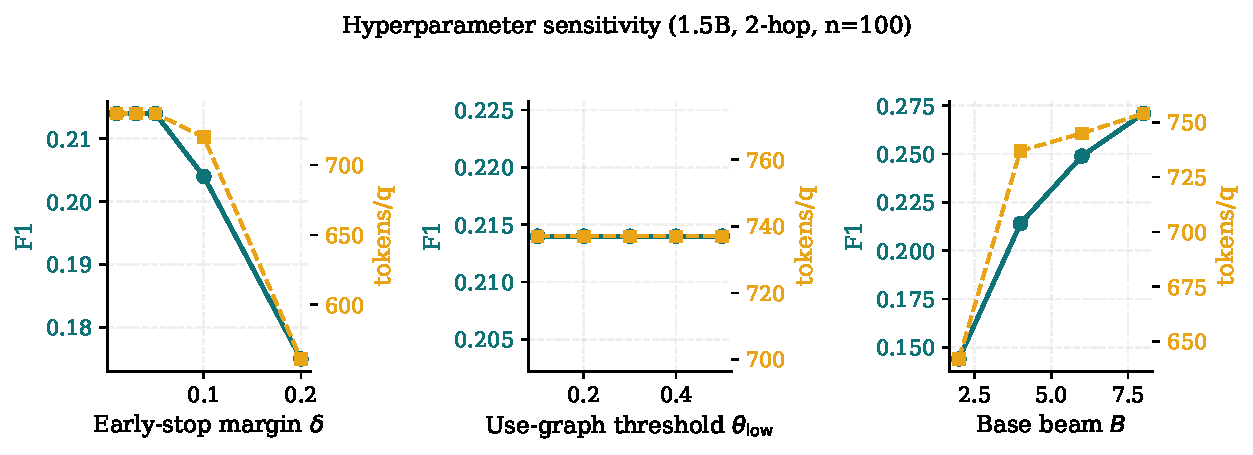
\includegraphics[width=0.98\columnwidth]{figures/fig_sensitivity.pdf}
\caption{Hyperparameter sensitivity (1.5B, 2-hop, $n{=}100$). F1 (teal, left axis) and tokens/query (amber, right axis) vs.\ each parameter. $\delta$ is stable on $[0.01,0.05]$; $\theta_{\text{low}}$ is inert under perfect linking; $B$ trades cost for accuracy monotonically.}
\label{fig:sensitivity}
\end{figure}

\subsubsection{Signal Quality: Is the Stopping Signal Safe?}
\label{sec:exp-signal}

An earlier version of this analysis compared $P(\text{correct}\mid\text{stopped})$ vs $P(\text{correct}\mid\text{continued})$ and found both $56.0\%$ at 7B/2-hop, concluding the stopped hops were uninformative. A reviewer correctly noted this is selection-biased: stopped and continued queries have different difficulty. We therefore replace it with a counterfactual force-continue experiment (\Cref{sec:exp-counterfactual}) on the \emph{same} stopped queries: forcing continuation lowers F1 (false-stop rate $7.8\%$, mean answer change $-0.032$), which is the correct test. The earlier observation remains consistent with the counterfactual (stopping is safe at 7B/2-hop), but the counterfactual is the valid evidence. The signal-quality AUROC (gain predicting ``force-continue helps'') is $0.503$ on all queries, near chance---consistent with the low false-stop rate. At 1.5B/3-hop the proxy breaks (stopped $21.2\%$ vs.\ continued $26.2\%$), consistent with the boundary analysis.

\subsubsection{Honest Boundaries}
\label{sec:exp-boundary}

We report settings where \method{} does \emph{not} win. \textbf{(i) Trivial queries:} at 1.5B/1-hop, \method{} lowers cost by $22\%$ but F1 drops $0.341{\to}0.332$. \textbf{(ii) Weak judge at depth:} at 1.5B/3-hop, No-Graph (F1 $0.109$) beats \method{} ($0.091$)---the 1.5B judge is too unreliable at depth 3. \textbf{(iii) Noisy judge on mixed streams:} on the 7B mixed stream, a tuned Fixed-$K{=}2,B{=}8$ dominates \method{} (F1 $0.474$ vs $0.395$), and even Oracle-depth is dominated (\Cref{sec:exp-mixed}). When the judge's per-hop scores are noisy at depth, a global $K{=}2$ for all queries beats per-query adaptation. \method{} recovers on the stronger 14B judge (\Cref{sec:exp-strong}).

\paragraph{The judge-quality scope condition.}
These boundaries share a cause: (D3)'s signal $t_k - t_{k-1}$ is a reliable proxy only when the judge's scores are reliable. The 14B result and the counterfactual (App.~E) bracket this: on a reliable judge, stopping is safe and beneficial; on a noisy judge at depth, it is not. This scope condition---not the controller---is the key determinant of when training-free GraphRAG adaptation succeeds. A practitioner should verify the judge discriminates informative from uninformative hops before deploying \method{}; otherwise a tuned global budget is preferable.

\paragraph{Absolute performance and scope.}
Our MetaQA F1 (0.18--0.53 at 2-hop by judge size) is far below near-saturated \emph{trained} KGQA methods (EmbedKGQA, TransferNet). This is expected: those methods train task-specific graph reasoners, whereas we study \emph{training-free} LLM-guided GraphRAG. Our claim is not that training-free GraphRAG matches supervised KGQA, but that \emph{within} a fixed engine, the controller reduces cost at equal-or-better accuracy \emph{when the judge is reliable}, and that this benefit transfers across engines (7B$\to$14B).
